\scanpage{71}
Structures sur catégorie \inserted{$(C)$} de \inserted{\unsure{(gr)}} motifs ($1/2$ \unsure{simples}) sur un ouvert $S\subset\operatorname{Spec}(\mathbb Z)$.

\margin{\figure{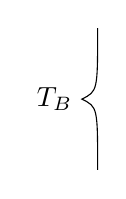
\begin{tikzpicture}[x=.2cm,y=.2cm]
\draw (1,9) .. controls (1,5) and (1,5) .. (0,4.5) .. controls (1,4) and (1,4) .. (1,0);
\node[left] at (0,4.5) {$T_B$};
\end{tikzpicture}}}
$T_B$ : foncteur de Betti (sur $\mathbb Q$) relatif : $\mathbb C$, \fbox{groupe $G$ sur $\mathbb Q$}
\[
T_\ell\simeq T_B\otimes_{\mathbb Q}\mathbb Q_\ell,
\qquad\text{réalisation $\ell$-adique (sur $\overline{\mathbb Q}\subset\mathbb C$)}
\]
\diagram{\begin{tikzcd}[column sep=small]
&\boxed{\begin{gathered}\begin{tikzcd}[column sep=small]
\pi=\operatorname{Gal}(\overline{\mathbb Q}/\mathbb Q)\arrow[r]&G(\mathbb Q_p)\\
\pi(p)=\operatorname{Gal}(\overline{\mathbb Q}_p/\mathbb Q_p)\arrow[u]&
\end{tikzcd}\end{gathered}}\arrow[r,bend left=20,no head]&\text{non ramifié dans }S-\{p\}\\
\pi(\infty)=\mathbb Z/2\mathbb Z\arrow[ur,bend left=20]& &p\in S\quad\text{($p$ premier fini ou $\infty$)}\arrow[ul,bend left=20,no head]
\end{tikzcd}}
\margin{\unsure{réalité} des autres \unsure{structures} $\unsure{\varphi^\infty|\mathbb C^\infty}$ resp \dots}
\[
\boxed{\begin{gathered}
\diagram{\begin{tikzcd}[column sep=large]
i_1^{(\infty)}\deleted{(\infty)},\ i_2^{(\infty)}\deleted{(\infty)}:\mathbb G_{m\mathbb C}\arrow[r,shift left]\arrow[r,shift right]&G(\mathbb C)\\
i_1^{(p)}\deleted{(p)},\ i_2^{(p)}\deleted{(p)}:\mathbb G_{m,\mathbb C^{(p)}}\deleted{\unsure{p}}\arrow[r,shift left]\arrow[r,shift right]&G(\mathbb C^{(p)})
\end{tikzcd}}
\end{gathered}}
\qquad\text{d'où}\quad
\left\{\begin{array}{l}
U^{(p)}\subset G_{\mathbb C^{(p)}}\\
U^{(\infty)}\subset G_{\mathbb C}\\
\text{(via }i_2^{(p)},i_2^{(\infty)}\text{)}
\end{array}\right.
\]
\figure{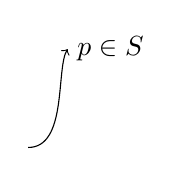
\begin{tikzpicture}[x=.5cm,y=.5cm]
\draw[->] (0,0) .. controls (1,0) and (.7,2) .. (1,2.5);
\node[right] at (1,2.5) {$p\in S$};
\end{tikzpicture}}

\margin{\figure{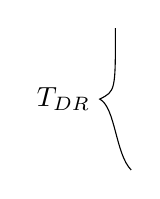
\begin{tikzpicture}[x=.2cm,y=.2cm]
\draw (1,9) .. controls (1,5) and (1,5) .. (0,4.5) .. controls (1,4) and (1,1) .. (2,0);
\node[left] at (0,4.5) {$T_{DR}$};
\end{tikzpicture}}}
$T_{DR}$ : foncteur de DeRham (sur $\mathbb Q$)

correspond à \fbox{torseur $P$ sous $G$}, groupe $G'$ sur $\mathbb Q$, $G'=\operatorname{ad}(P)=G^P$.

\uline{filtré}, i.e. on a une famille d'hom
\diagram{\begin{tikzcd}j_2:\mathbb G_{m\mathbb Q}\arrow[r,no head]&G'\end{tikzcd}}
défini mod conjugaison par les elts du groupe unipotent associé $U'\subset G'$ ($\Rightarrow$ torseur $R$ sur $U'$).

$\forall p\in S$, $p$ premier fini, on a
\[
\boxed{\begin{array}{l}F_p\in G'(\mathbb Q_p)\\F_\infty\in G'(\mathbb R)\end{array}}
\quad\text{(Frobenius)}
\]
\inserted{d'ordre $2$}

\margin{\figure{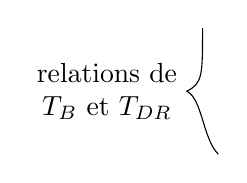
\begin{tikzpicture}[x=.2cm,y=.2cm]
\draw (1,8) .. controls (1,5) and (1,4.5) .. (0,4) .. controls (1,3.5) and (1,1) .. (2,0);
\node[left,align=center] at (0,4) {relations de\\$T_B$ et $T_{DR}$};
\end{tikzpicture}}}
\deleted{Etant \unsure{donné}} \deleted{$\unsure{\rho}$}
\[
\boxed{\rho^{(\infty)}\in P(\mathbb C)}
\]
transformant la classe des $\unsure{j'_{2\mathbb C}|j_{2\mathbb C}}$ en celle de $i_2^{(\infty)}$.

Pour tt $\unsure{j_2^*|j'_2}\in U'$, et tout $\lambda\in\mathbb C^p(1)^*$, on obtient
\[
\boxed{\rho^{(p)}(j_2,\lambda)\in P(\mathbb C^p)}
\]
transformant le \uuline{$j_2$ en $i_2$}

i.e.
\[
\left\{\begin{gathered}
\diagram{\begin{tikzcd}
\mathbb C^{(p)}(1)^*\times U'(\unsure{\mathbb C^p|\mathbb C})\arrow[r,no head]&P(\mathbb C^p)
\end{tikzcd}}\\
\boxed{\begin{gathered}\diagram{\begin{tikzcd}
\mathbb G_{m\mathbb C^p}\arrow[r,"i_2^{(p)}"]&\unsure{G_{\mathbb C^p}|G'_{\mathbb C^p}}&G'_{\mathbb C^p}\supset U'_{\mathbb C^p}
\end{tikzcd}}\end{gathered}}
\end{gathered}\right.
\]
et compatibilité aux opérations de

\begin{tabular}{ll}
a)&$\mathbb C^{(p)*}\times U'(\mathbb C^p)$\\
b)&$\pi(p)=\operatorname{Gal}(\overline{\mathbb Q}_p/\mathbb Q_p)$
\end{tabular}
\mspage{70}
